\newcommand{\tdplotmainfig}{%
\ifpdf
%Angle Definitions
%-----------------
%
%set the plot display orientation
%synatax: \tdplotsetdisplay{\theta_d}{\phi_d}
\tdplotsetmaincoords{60}{110}
%
%define polar coordinates for some vector
%TODO: look into using 3d spherical coordinate system
\pgfmathsetmacro{\rvec}{.8}
\pgfmathsetmacro{\thetavec}{30}
\pgfmathsetmacro{\phivec}{60}
%
%start tikz picture, and use the tdplot_main_coords style to implement the display coordinate transformation provided by 3dplot
\begin{tikzpicture}[scale=3,tdplot_main_coords]

	%set up some coordinates 
	%-----------------------
	\coordinate (O) at (0,0,0);

	%determine a coordinate (P) using (r,\theta,\phi) coordinates.  This command also determines (Pxy), (Pxz), and (Pyz): the xy-, xz-, and yz-projections of the point (P).
	%synatax: \tdplotsetcoord{Coordinate name without parentheses}{r}{\theta}{\phi}
	\tdplotsetcoord{P}{\rvec}{\thetavec}{\phivec}

	%draw figure contents
	%--------------------

	%draw the main coordinate system axes
	\draw[thick,->] (0,0,0) -- (1,0,0) node[anchor=north east]{$x$};
	\draw[thick,->] (0,0,0) -- (0,1,0) node[anchor=north west]{$y$};
	\draw[thick,->] (0,0,0) -- (0,0,1) node[anchor=south]{$z$};

	%draw a vector from origin to point (P) 
	\draw[-stealth,color=red] (O) -- (P);

	%draw projection on xy plane, and a connecting line
	\draw[dashed, color=red] (O) -- (Pxy);
	\draw[dashed, color=red] (P) -- (Pxy);

	%draw the angle \phi, and label it
	%syntax: \tdplotdrawarc[coordinate frame, draw options]{center point}{r}{angle}{label options}{label}
	\tdplotdrawarc{(O)}{0.2}{0}{\phivec}{anchor=north}{$\phi$}


	%set the rotated coordinate system so the x'-y' plane lies within the "theta plane" of the main coordinate system
	%syntax: \tdplotsetthetaplanecoords{\phi}
	\tdplotsetthetaplanecoords{\phivec}

	%draw theta arc and label, using rotated coordinate system
	\tdplotdrawarc[tdplot_rotated_coords]{(0,0,0)}{0.5}{0}{\thetavec}{anchor=south west}{$\theta$}

	%draw some dashed arcs, demonstrating direct arc drawing
	\draw[dashed,tdplot_rotated_coords] (\rvec,0,0) arc (0:90:\rvec);
	\draw[dashed] (\rvec,0,0) arc (0:90:\rvec);

	%set the rotated coordinate definition within display using a translation coordinate and Euler angles in the "z(\alpha)y(\beta)z(\gamma)" euler rotation convention
	%syntax: \tdplotsetrotatedcoords{\alpha}{\beta}{\gamma}
	\tdplotsetrotatedcoords{\phivec}{\thetavec}{0}

	%translate the rotated coordinate system
	%syntax: \tdplotsetrotatedcoordsorigin{point}
	\tdplotsetrotatedcoordsorigin{(P)}

	%use the tdplot_rotated_coords style to work in the rotated, translated coordinate frame
	\draw[thick,tdplot_rotated_coords,->] (0,0,0) -- (.5,0,0) node[anchor=north west]{$x'$};
	\draw[thick,tdplot_rotated_coords,->] (0,0,0) -- (0,.5,0) node[anchor=west]{$y'$};
	\draw[thick,tdplot_rotated_coords,->] (0,0,0) -- (0,0,.5) node[anchor=south]{$z'$};

	%WARNING:  coordinates defined by the \coordinate command (eg. (O), (P), etc.) cannot be used in rotated coordinate frames.  Use only literal coordinates.  

	%draw some vector, and its projection, in the rotated coordinate frame
	\draw[-stealth,color=blue,tdplot_rotated_coords] (0,0,0) -- (.2,.2,.2);
	\draw[dashed,color=blue,tdplot_rotated_coords] (0,0,0) -- (.2,.2,0);
	\draw[dashed,color=blue,tdplot_rotated_coords] (.2,.2,0) -- (.2,.2,.2);

	%show its phi arc and label
	\tdplotdrawarc[tdplot_rotated_coords,color=blue]{(0,0,0)}{0.2}{0}{45}{anchor=north west,color=black}{$\phi'$}

	%change the rotated coordinate frame so that it lies in its theta plane.  Note that this overwrites the original rotated coordinate frame
	%syntax: \tdplotsetrotatedthetaplanecoords{\phi'}
	\tdplotsetrotatedthetaplanecoords{45}

	%draw theta arc and label
	\tdplotdrawarc[tdplot_rotated_coords,color=blue]{(0,0,0)}{0.2}{0}{55}{anchor=south west,color=black}{$\theta'$}

\end{tikzpicture}
\fi
}

\newcommand{\threedcoord}[2]{%
\ifpdf
\tdplotsetmaincoords{#1}{#2}
\begin{tikzpicture}[tdplot_main_coords]
	\draw[thick,->] (0,0,0) -- (1,0,0) node[anchor=north east]{$x$};
	\draw[thick,->] (0,0,0) -- (0,1,0) node[anchor=north west]{$y$};
	\draw[thick,->] (0,0,0) -- (0,0,1) node[anchor=south]{$z$};
\end{tikzpicture}
\fi
}

\newcommand{\threedrotcoordsystem}{%
\ifpdf
\tdplotsetmaincoords{50}{140}
\begin{tikzpicture}[scale=5,tdplot_main_coords]
	\draw[thick,->] (0,0,0) -- (1,0,0) node[anchor=north east]{$x$};
	\draw[thick,->] (0,0,0) -- (0,1,0) node[anchor=north west]{$y$};
	\draw[thick,->] (0,0,0) -- (0,0,1) node[anchor=south]{$z$};

	\tdplotsetrotatedcoords{34}{26}{12}

	\draw[thick,color=blue,tdplot_rotated_coords,->] (0,0,0) -- (.5,0,0) node[anchor=north east]{$x'$};
	\draw[thick,color=blue,tdplot_rotated_coords,->] (0,0,0) -- (0,.5,0) node[anchor=north west]{$y'$};
	\draw[thick,color=blue,tdplot_rotated_coords,->] (0,0,0) -- (0,0,.5) node[anchor=south]{$z'$};
	
\end{tikzpicture}
\fi
}

\newcommand{\threedconventions}{%
\ifpdf
\tdplotsetmaincoords{50}{110}
\begin{tikzpicture}[scale=2,tdplot_main_coords]
	\draw[thick,->] (0,0,0) -- (1,0,0) node[anchor=north east]{$x$};
	\draw[thick,->] (0,0,0) -- (0,1,0) node[anchor=north west]{$y$};
	\draw[thick,->] (0,0,0) -- (0,0,1) node[anchor=south]{$z$};

	\draw[color=blue] (0,0,0) -- (.5,.5,0);

	\draw[color=blue,->] (.5,0,0) arc (0:45:.5);	
\end{tikzpicture}
\fi
}


\newcommand{\threedalphabetagamma}{%
\ifpdf
\beginpgfgraphicnamed{Figures/alphabetagamma}
\tdplotsetmaincoords{50}{140}
%
\begin{tikzpicture}[scale=2,tdplot_main_coords]
	\draw[thick,->] (0,0,0) -- (1,0,0) node[anchor=north east]{$x$};
	\draw[thick,->] (0,0,0) -- (0,1,0) node[anchor=north west]{$y$};
	\draw[thick,->] (0,0,0) -- (0,0,1) node[anchor=south]{$z$};

	\tdplotsetrotatedcoords{0}{0}{30}

	\draw[thick,color=red,tdplot_rotated_coords,->] (0,0,0) -- (.7,0,0) node[anchor=north]{$x'$};
	\draw[thick,color=green!50!black,tdplot_rotated_coords,->] (0,0,0) -- (0,.7,0) node[anchor=west]{$y'$};
	\draw[thick,color=blue,tdplot_rotated_coords,->] (0,0,0) -- (0,0,.7) node[anchor=west]{$z'$};
	
	\tdplotdrawarc[color=orange!50!black]{(0,0,0)}{.4}{0}{30}{anchor=north east}{$\gamma$}
\end{tikzpicture}
%
\begin{tikzpicture}[scale=2,tdplot_main_coords]
	\draw[thick,->] (0,0,0) -- (1,0,0) node[anchor=north east]{$x$};
	\draw[thick,->] (0,0,0) -- (0,1,0) node[anchor=north west]{$y$};
	\draw[thick,->] (0,0,0) -- (0,0,1) node[anchor=south]{$z$};

	\tdplotsetrotatedcoords{0}{0}{30}

	\draw[dashed,color=red,tdplot_rotated_coords] (0,0,0) -- (.5,0,0);
	\draw[dashed,color=green!50!black,tdplot_rotated_coords] (0,0,0) -- (0,.5,0);
	\draw[dashed,color=blue,tdplot_rotated_coords] (0,0,0) -- (0,0,.5);

	\tdplotsetrotatedcoords{0}{40}{30}

	\draw[thick,color=red,tdplot_rotated_coords,->] (0,0,0) -- (.7,0,0) node[anchor=north]{$x'$};
	\draw[thick,color=green!50!black,tdplot_rotated_coords,->] (0,0,0) -- (0,.7,0) node[anchor=west]{$y'$};
	\draw[thick,color=blue,tdplot_rotated_coords,->] (0,0,0) -- (0,0,.7) node[anchor=south]{$z'$};
	
	\tdplotsetthetaplanecoords{0}
	\tdplotdrawarc[tdplot_rotated_coords,color=orange!50!black]{(0,0,0)}{.4}{0}{40}{anchor=south}{$\beta$}

\end{tikzpicture}
%
\begin{tikzpicture}[scale=2,tdplot_main_coords]
	\draw[thick,->] (0,0,0) -- (1,0,0) node[anchor=north east]{$x$};
	\draw[thick,->] (0,0,0) -- (0,1,0) node[anchor=north west]{$y$};
	\draw[thick,->] (0,0,0) -- (0,0,1) node[anchor=south]{$z$};

	\tdplotsetrotatedcoords{0}{40}{30}

	\draw[dashed,color=red,tdplot_rotated_coords] (0,0,0) -- (.5,0,0);
	\draw[dashed,color=green!50!black,tdplot_rotated_coords] (0,0,0) -- (0,.5,0);
	\draw[dashed,color=blue,tdplot_rotated_coords] (0,0,0) -- (0,0,.5);

	\tdplotsetrotatedcoords{60}{0}{0}
	\draw[dotted,color=blue,tdplot_rotated_coords] (0,0,0) -- (.4,0,0);
	\tdplotsetrotatedcoords{60}{40}{30}

	\draw[thick,color=red,tdplot_rotated_coords,->] (0,0,0) -- (.7,0,0) node[anchor=north]{$x'$};
	\draw[thick,color=green!50!black,tdplot_rotated_coords,->] (0,0,0) -- (0,.7,0) node[anchor=west]{$y'$};
	\draw[thick,color=blue,tdplot_rotated_coords,->] (0,0,0) -- (0,0,.7) node[anchor=south]{$z'$};


	\tdplotdrawarc[color=orange!50!black]{(0,0,0)}{.2}{0}{60}{anchor=north east}{$\alpha$}
\end{tikzpicture}
\endpgfgraphicnamed
\fi
}

\newcommand{\threedthetaarc}{%
\ifpdf
%
\tdplotsetmaincoords{70}{110}
%
\begin{tikzpicture}[scale=5,tdplot_main_coords]
	\draw[thick,->] (0,0,0) -- (1,0,0) node[anchor=north east]{$x$};
	\draw[thick,->] (0,0,0) -- (0,1,0) node[anchor=north west]{$y$};
	\draw[thick,->] (0,0,0) -- (0,0,1) node[anchor=south]{$z$};

	\tdplotsetcoord{P}{.8}{50}{70}

	%draw a vector from origin to point (P) 
	\draw[-stealth,color=red] (O) -- (P);

	%draw projection on xy plane, and a connecting line
	\draw[dashed, color=red] (O) -- (Pxy);
	\draw[dashed, color=red] (P) -- (Pxy);


	\tdplotsetthetaplanecoords{70}

	\draw[tdplot_rotated_coords,color=blue,thick,->] (0,0,0) -- (.2,0,0) node[anchor=east]{$x'$};
	\draw[tdplot_rotated_coords,color=blue,thick,->] (0,0,0) -- (0,.2,0) node[anchor=north]{$y'$};
	\draw[tdplot_rotated_coords,color=blue,thick,->] (0,0,0) -- (0,0,.2) node[anchor=west]{$z'$};


	\tdplotdrawarc[tdplot_rotated_coords,color=orange!50!black]{(0,0,0)}{.4}{0}{50}{anchor=north east}{$\theta$}
\end{tikzpicture}
\fi
}

\newcommand{\threedparamplot}{%
\ifpdf
%
\beginpgfgraphicnamed{Figures/threedparamplot}
\tdplotsetmaincoords{70}{110}
%
\begin{tikzpicture}[scale=2,tdplot_main_coords]
	\draw[thick,->] (0,0,0) -- (1,0,0) node[anchor=north east]{$x$};
	\draw[thick,->] (0,0,0) -- (0,1,0) node[anchor=north west]{$y$};
	\draw[thick,->] (0,0,0) -- (0,0,1) node[anchor=south]{$z$};

	\pgfplothandlerlineto
	\pgfplotfunction{\thetaen}{0,6,...,360}{%
		\pgfpointxyz{cos(\thetaen)}%
			{sin(\thetaen)}%
			{\thetaen/400}
	}
	\pgfusepath{stroke}

\end{tikzpicture}
\endpgfgraphicnamed
\fi
}

\newcommand{\threedsurfaceplot}{%
\ifpdf
\beginpgfgraphicnamed{Figures/threedsurfaceplot}
%
\tdplotsetmaincoords{70}{135}
%
\begin{tikzpicture}[scale=3,line join=bevel,tdplot_main_coords, fill opacity=.6]

\tdplotsphericalsurfaceplot[parametricfill]{72}{36}%
%{0.3}{black}{red}%
%{0.5*sin(\tdplottheta)*sin(\tdplottheta)}{black}{red}%
%{0.5*sin(\tdplottheta)*sin(\tdplottheta)*sin(\tdplotphi)*sin(\tdplotphi)}{black}{red}%
%{0.5*cos(\tdplottheta)*cos(\tdplottheta)}{black}{red}%
%{0.25*cos(\tdplottheta)}{black}{red}%
{(sin(\tdplottheta)*cos(\tdplottheta))}{black}{\tdplotphi}%
%{ .15*(3*cos(\tdplottheta)*cos(\tdplottheta) - 1 )^2}{black}{\tdplotphi}
	{\draw[color=black,thick,->] (0,0,0) -- (1,0,0) node[anchor=north east]{$x$};}%
	{\draw[color=black,thick,->] (0,0,0) -- (0,1,0) node[anchor=north west]{$y$};}%
	{\draw[color=black,thick,->] (0,0,0) -- (0,0,1) node[anchor=south]{$z$};}%

\end{tikzpicture}
\endpgfgraphicnamed
\fi
}

\newcommand{\colortest}{%
\ifpdf
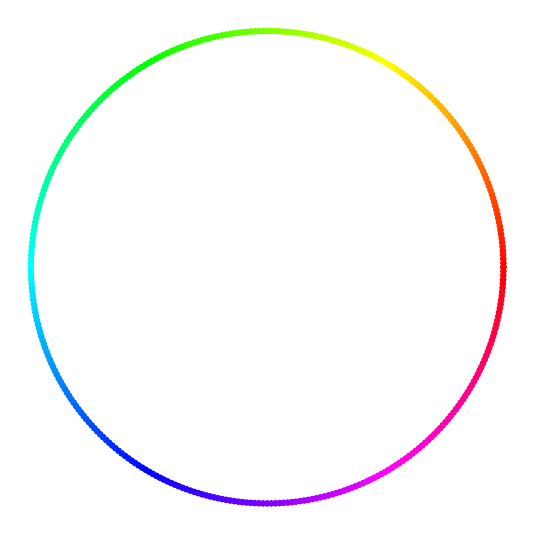
\begin{tikzpicture}
	\foreach \thetawheel in {0,1,...,360}
	{
		%\tdplotcalcrgb{\thetawheel}
		\pgfmathdivide{\thetawheel}{360}
		\definecolor{tdplotcolor}{hsb}{\pgfmathresult, 1, 1}
		\color{tdplotcolor}
		\filldraw(\thetawheel:3) circle (1pt);
	}
\end{tikzpicture}
\fi
}
